Negli algoritmi visti fin'ora, per trovare la policy adatta ($a = \pi(s)$ dove con $\pi$ indichiamo appunto la \textit{policy}) siamo sempre andati ad utilizzare una funzione approssimata $Q_{\pi^*}(s,a)$, la quale permetteva all'agente di scegliere quale fosse l'azione migliore da compiere, sia nel caso di azioni discrete, sia nel caso di azioni continue che discrete ()come si vede in figura ~\ref{fig:Q_function_utility}) andando poi a selezionare l'azione in grado di massimizzare l'output.

\begin{figure}[!h]
	\centering
	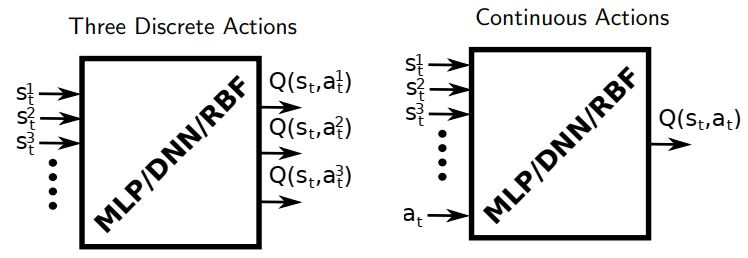
\includegraphics[width=0.8\textwidth]{Immagini/Q_function_utility.JPG}
	\caption{Valutazione della funzione sulla base della Q-values}
	\label{fig:Q_function_utility}
\end{figure}

La domanda che ci poniamo è: \textit{possiamo trovare la policy direttamente} partendo dallo stato attuale ($s_t$) e ottenendo appunto $a_t$?

La risposta è si.

\begin{figure}[!h]
	\centering
	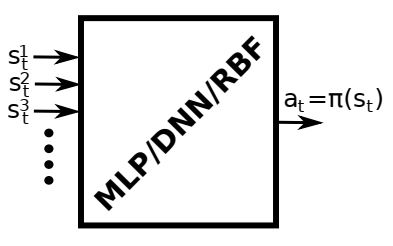
\includegraphics[width=0.5\textwidth]{Immagini/No_Q_function.JPG}
	\caption{Valutazione della funzione \textit{non} basandosi sulla Q-values}
	\label{fig:NO_Q_function_utility}
\end{figure}
Questo concetto, mostrato in maniera molto diretta nella figura ~\ref{fig:NO_Q_function_utility}, è quello che nella letteratura del RL viene chiamato come metodo di \textit{policy search}, il quale permette appunto di stimare la polici ottimale ($\pi^*(a|s)$) invece di cercare il valore ottimo per la funzione $Q^*(s,a))$: questo nuovo approccio presenta innumerevoli vantaggi rispetto agli algoritmi mostrati in precedenza, in particolare:
\begin{itemize}
	\item Policies ottimali, scelte tramite algoritmi di questo tipo, presentano un numero di parametri minore rispetto al valore ottimale della q-functions (\textit{curse of dimensionality})
	\item Processo di learn più veloce (e questo è anche dimostrato dai grafici presenti all'interno di questa documentazione)
	\item Offre la possibilità di utilizzare policies sia deterministiche che stocastiche (\textit{noisly})
\end{itemize}

\textit{E cosa cerchiamo di ottimizzare in questo nuovo contesto?}
I metodi di policy search vanno ad ottimizzare l'indice $J(\theta)$, dove $\theta$ rappresenta il vettore dei pesi; è possibile realizzare questa ottimizzazione utilizzando differenti metodi:
\begin{itemize}
	\item Gradient free methods:
	\begin{itemize}
		\item Evolutionary computation
		\item Simulated annealing
		\item Hill climbing
	\end{itemize}
	\item \textbf{Gradient based methods} (\textit{policy gradient methods}):
	\begin{itemize}
		\item  Gradient estimation 
		\item Optimization algorithm
	\end{itemize}
\end{itemize}

I passi principali che sono stati implementati, sono
\begin{itemize}
	\item Implementare la dinamica del carrello (di cui non si riporta la trattazione) e una funzione per simulare i roll-outs (sotto sezione ~\ref{sec:rollout}) che forniscono il reward di ritorno;
	\item Utilizzare una \textit{Radial Basis Function} (RBF network - sotto sezione ~\ref{sec:RBF}) per approssimare l'apprendimento, ovvero per ottenere $a = \pi(s,W) = W^T\Phi(s,a)$
	\item Implementare l'algoritmo alla differenze finite (FD) per apprendere i pesi della policy
\end{itemize}

\subsection{Approccio \textit{Policy gradient estimation}}
Come già sottolineato in precedenza andremo a basarci su un algoritmo \textit{gradient based}, nello specifico l'agoritmo alla differenze finite, il quale, in ambito matematico, rappresenta una strategia utilizzata per risolvere numericamente equazioni differenziali che si basa sull'approssimazione delle derivate con equazioni alle differenze finite.

Questa approssimazione andiamo ad utilizzare per effettuare un'operazione di minimizzazione (anche locale) sulla funzione $J(\theta) = V_\pi(s)$ \label{eq:J_function_to_minimize}: l'approccio che si è deciso di seguire non è però quello classico, ma bensì una strada alternativa, in cui, fornita una policy parametrizzata $\pi(a|s,\theta)$, possiamo calcolare $J(\theta)$ simulando l'environment come un \textit{Markov Decision Process}, la funzione $J(\theta)$. 

In particolare:
\begin{itemize}
	\item Invece di calcolare $\partial V / \partial\phi_i$ separatamente (passaggio che verrebbe naturale dopo aver definito $J(\theta)$ in \ref{eq:J_function_to_minimize}), andiamo ad ottenere un vettore random $\delta ~ N (0, \sigma^2)$.
	Nel codice questa parte è stata implementata in questo modo:
	\begin{lstlisting}
	# Variance of the random Gaussian perturbation of the parameters
	variance_of_perturbation = 0.1 
	# random parameter 	variation (Gaussian)
	delta = variance_of_perturbation * np.random.randn(numberOfCentrum, 1) 
	\end{lstlisting}
	\item Il vettore randomico generato in precedenza lo utilizzeremo poi per calcolare, tramite la tecnica definita \textit{roll-out} (sezione ~\ref{sec:rollout}), due valori della funzione J ($J_+, J_-$)
	
	TODO........
	
\end{itemize}

\subsubsection{RBF network}
\label{sec:RBF}
\subsubsection{\textit{Phi} function}
\subsubsection{Rollout}
\label{sec:rollout}

\begin{figure}[!h]
	\centering
	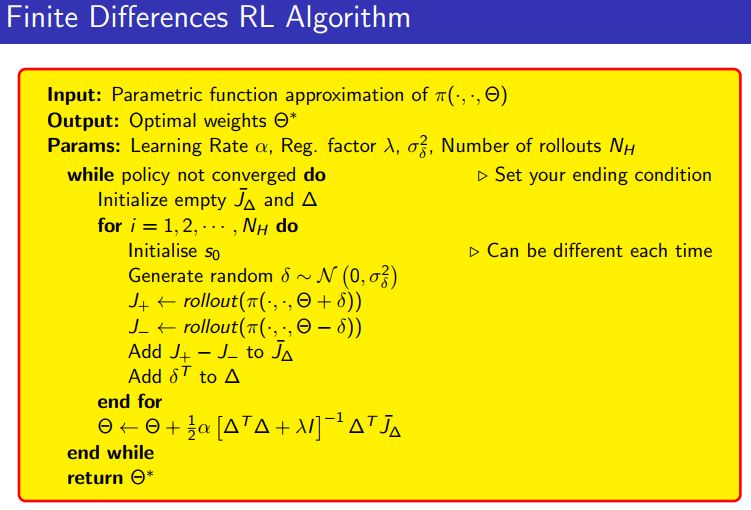
\includegraphics[width=\textwidth]{Immagini/FD_Algorithm.JPG}
	\caption{\textit{Finite Differences} algoritmo implementato}
	\label{fig:Reward_FD}
\end{figure}



Reward con un batch di 10 trial con 70 iterazioni: ogni iterazione può essere eseguita per un massimo di 10 s, se l'esecuzione non fallisce prima (ovvero il pole cade fuori dal range angolare imposto).

\subsection{Result}
TODO: confronto anche con tempo di esecuzione del codice scritto in Matlab.
\begin{figure}[!h]
	\centering
	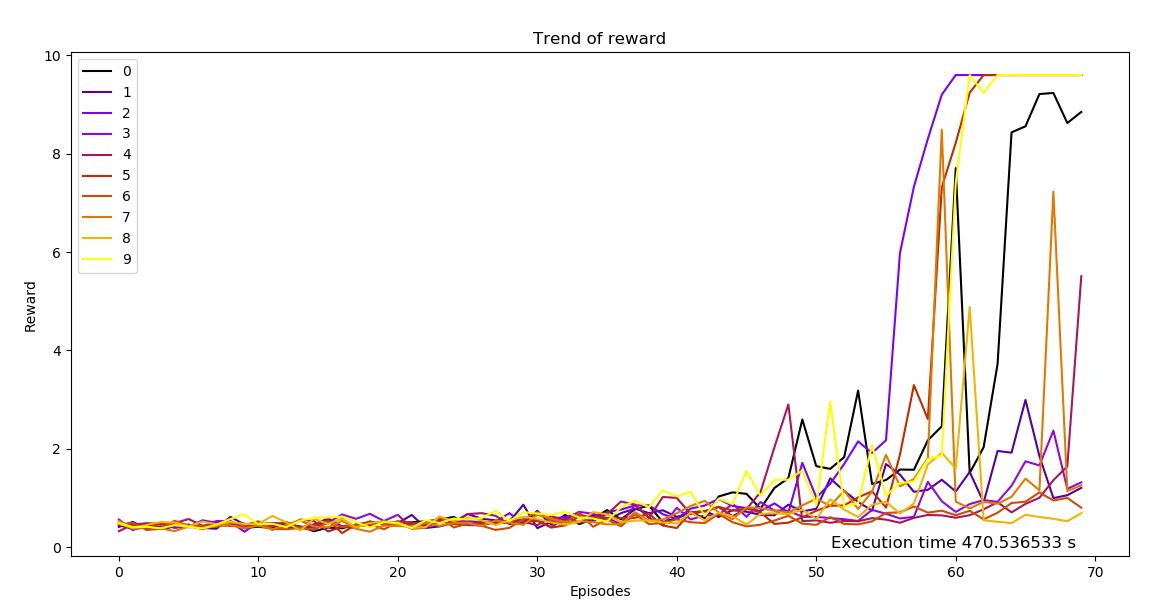
\includegraphics[width=\textwidth]{Immagini/Reward_FD.JPG}
	\caption{Reward \textit{Finite Differences}}
	\label{fig:Reward_FD}
\end{figure}

\newpage